\chapter{Electromagnetismo, ondas, antenas}

\section{Análisis vectorial y campos en el espacio vacío}

Recordemos los símbolos empleados para las variables independientes en los tres sistemas principales:

\begin{enumerate}
    \item Coordenadas $(x,y,z)$
    \item Coordenadas $(\rho, \phi, z)$
    \item Coordenadas $(r, \theta, \phi)$
\end{enumerate}

\subsection{Elementos diferenciales de espacio}

En el proceso de integración en el espacio se usan los elementos diferenciales de volumen, superficie y línea. Un elemento deiferencial de volumen $dv$ se genera en la proximidad de un pinto $P(u_1,u_2,u_3)$ del espacio, mediante los desplazamientos $dl_1, dl_2$ y $dl_3$ de las superficies coordenadas, a través de los cambios diferenciales $du_1, du_2$ y $du_3$ en las variables coordenadas. Por tanto, un elemento de volumen $dv$ se representa en las coordenadas ortogonales generalizadas mediante el priducto de los elementos diferenciales de longitud.

\begin{equation*}
dv = dl_1 \ dl_2 \ dl_3
\end{equation*}

La relación de los elementos de longitud a cambios diferenxiales en las variables coordenadas $u_1, u_2$ y $u_3$ proviene de las relaciones  

\begin{eqnarray*}
dl_1 = h_1 du_1 \\
dl_2 = h_2 du_2 \\
dl_3 = h_3 du_3
\end{eqnarray*}

de modo que el elemento de volumen queda como sigue

\begin{equation*}
dv = h_1 h_2 h_3 du_1 du_2 du_3
\end{equation*}

Los coeficientes $h_i$ se conocen como coeficientes métricos, los cuales son necesarios para darles dimensiones de longitud. Los elementos de longitud se pueden determinar de la siguiente manera

\begin{eqnarray*}
dl_1 = dx \\
dl_2 = dy \\
dl_3 = dz \\
h_1 = h_2 = h_3 = 1
\end{eqnarray*}

\begin{figure}[H]
    \centering
    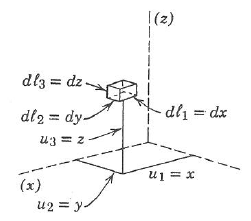
\includegraphics{Waves/waves_f1.png}
\end{figure}

Para las coordenadas cilíndricas tenemos que 

\begin{figure}[H]
    \centering
    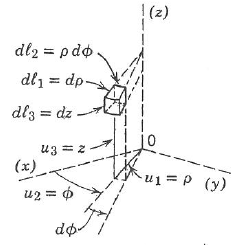
\includegraphics{Waves/waves_f2.png}
\end{figure}

El elemento $dl_2$ corresponde a la longitud de arco de radio $\rho$ y ángulo $d \phi$, de modo que queda

\begin{eqnarray*}
dl_1 = d\rho \\
dl_2 = \rho d\phi \\
dl_3 = dz \\
h_1 = 1 \\
h_2 = \rho \\
h_3 = 1
\end{eqnarray*}

Y para las coordenadas esféricas 
\begin{figure}[H]
    \centering
    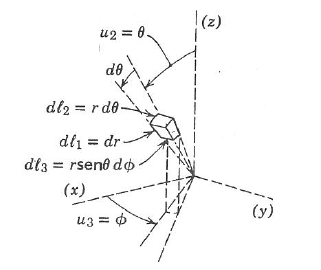
\includegraphics{Waves/waves_f3.png}
\end{figure}

La longitud de arco que corresponde a $dl_3$ corresponde a la proyección del elemento volumétrico sobre el plano $xy$, el radio corresponderá a $r \sin \theta$ y la longitud de arco $r \sin \theta$, por tanto 

\begin{eqnarray*}
dl_1 = d r \\
dl_2 = r d\theta \\
dl_3 = r \sin \theta d \phi \\
h_1 = 1 \\
h_2 = r \\
h_3 = r \sin \theta
\end{eqnarray*}

Finalmente los elementos de volumen quedan

\begin{eqnarray*}
dv = dx \ dy \ dz \\
dv = \rho \ d\rho \ d \phi \ d z \\
dv = r^2 \sin \theta \ dr \ d \theta \ d \phi
\end{eqnarray*}

Un elemento $ds$ de una duperficie en el espacio se puede dejar en su forma escalar $ds$ pero si se desea se puede dar una caracterización vectorial $d \mathbf{s}$. Para el ejemplo de coordenadas esféricas, la forma escalar del elemento de superficie sería

\begin{equation*}
ds = r^2 \sin \theta d \theta \ d \phi
\end{equation*}

la condición vectorial se otorga multiplicando este elemento de superficie con un vector unitario normal al elemento de superficie. 

\begin{equation*}
d \mathbf{s} = \mathbf{a}_{r} ds = \mathbf{a}_{r} r^2 \sin \theta d \theta \ d \phi
\end{equation*}



\subsection{Vector de posición}

Para cada punto en el espacio se puede hacer una notación vectorial, el cual corresponde a un vector desde el origen hasta el punto en cuestión. Para las coordenadas rectangulares,

\begin{equation*}
\mathbf{r} = \mathbf{a}_x x + \mathbf{a}_y y + \mathbf{a}_z z
\end{equation*}

para las coordenadas cilíndricas,

\begin{equation*}
\mathbf{r} = \mathbf{a}_{\rho} \rho + \mathbf{a}_z z
\end{equation*}

y en las coordenadas cilíndricas

\begin{equation*}
\mathbf{r} = \mathbf{a}_r r
\end{equation*}

Una forma de realizar notación de puntos en el espacio es mediante el vector $\mathbf{r}$ es $P(\mathbf{r})$. El elemento diferencial de longitud que separa los puntos $P(\mathbf{r})$ y $P(\mathbf{r} + d \mathbf{r})$ se denota con el elemento diferencial $d \mathbf{r}$ y se define de la siguiente manera:

\begin{equation*}
d \mathbf{r} = \mathbf{a}_1 d l_1 + \mathbf{a}_2 d l_2 + \mathbf{a}_3 d l_3
\end{equation*}

Se forma un paralelepípedo cuyos vértices opuestos está formado por el vector diferencial, y la longitud de este vector está dada por 

\begin{equation*}
d l = \left( (h_1 d u_1)^2 + (h_2 d u_2)^2 + (h_3 d u_3)^2 \right)^{\frac{1}{2}}
\end{equation*}

Como ejemplo, para las coordenadas esféricas, el elemento de línea será

\begin{equation*}
d \mathbf{r} = d \mathbf{l} = \mathbf{a}_r d r + \mathbf{a}_\theta r d \theta + \mathbf{a}_\phi r \sin \theta d \phi  
\end{equation*}

y su longitud es

\begin{equation*}
dl = \sqrt{(dr)^2 + (r d\theta)^2 + (r \sin \theta \ d \phi)^2}
\end{equation*}

\subsection{Integración de vectores}

 Es conveniente examinar con cuidado el integrando de la integral vectorial, porque puede ser un escalar o un vector, por ejemplo la integral de línea 

\begin{equation*}
\int_{l} \mathbf{A} \cdot \mathbf{B} \ d l  
\end{equation*}

 la integral de superficie

\begin{equation*}
\int_S (\mathbf{A} \times \mathbf{B}) \cdot d\mathbf{s}
\end{equation*}

y la integral de volumen

\begin{equation*}
\int_V \mathbf{A} \times \mathbf{B} dv
\end{equation*}

Son elementos escalares, porque tiene integrandos escalares. Por su parte las siguientes integrales

\begin{eqnarray*}
\int_l \mathbf{G} \ d\mathbf{l} \\
\int_S \mathbf{H} \times d \mathbf{s} \\
\int_V \mathbf{J} \times \mathbf{K} \ dv
\end{eqnarray*}

Posee integrandos vectoriales y por tanto sus resultados son vectoriales.

Un ejemplo de gran utilidad es la integral escalar de línea 

\begin{equation*}
\int_l \mathbf{F} \times d \mathbf{l} = \int_l F dl \cos \theta
\end{equation*}

La integral de trabajo. Para las coordenadas generalizadas podemos determinar esta integral de la siguiente manera

\begin{eqnarray*}
\int \mathbf{F} \times d \mathbf{l} &=& \int_l F_1 dl_1 + \int_l F_2 d l_2 + \int_l F_3 d l_3 \\
&=& \int_l F_1 h_1 \ du_1 + \int_l F_2 h_2 \ du_2 + \int_l F_3 h_3 \ du_3
\end{eqnarray*}

\subsection{Cargas eléctricas, corrientes y sus densidades}

Desde el punto de vista del electromagnetismo clásico, se considera a un conjunto de cargas eléctricas como si fuera capaz de dividirse indefinidamente, de manera que la densidad volumétrica de carga, indicada por el símbolo $\rho_v$ y se define:

\begin{equation*}
\rho_v = \frac{\Delta q}{\Delta v} \text{C}/\text{m}^3
\end{equation*}

Dado que la carga que reside dentro de un volumen puede variar de un punto a otro de la región, y también puede variar con el tiempo, la densidad de carga es un campo escalar y se puede escribir como $\rho_v(u_1,u_2,u_3,t)$ o $\rho_v(\mathbf{r},t)$.

También se puede describir la densidad de carga en superficies o en caminos concretos como densidad superficial de carga y densidad lineal de carga $\rho_s$ y $\rho_l$. Las cargas pueden ser  positivas o negativas, y la carga neta siempre será la suma de las cargas positivas y las negativas. 

La cantidad total de carga contenida en una región de volumen, superficie o línea se puede determinar como la integral del campo densidad a lo largo de la región.

\begin{equation*}
q = \int_v \rho_v \ dv
\end{equation*}

Teniendo un campo vectorial en el espacio, podemos definir cualquier superficie y medir la cantidad de líneas del campo que atraviesa dicha superficie. Las líneas de flujo neto $\psi$ que pasan a través de $S$ pueden ser una medida de alguna cantidad física. La cantidad diferencial de flujo $d \psi$ que pasa a través de cualquier elemento superficial $ds$ en el espacio, se define como el producto punto $\mathbf{F} \cdot d \mathbf{s}$. Como consecuencia el flujo neto del campo $\mathbf{F}$ a través de la superficie $S$ es la suma de todos los flujos diferenciales

\begin{equation*}
\psi = \int_S \mathbf{F} \cdot d \mathbf{s}
\end{equation*}

Si la superficie es cerrada, entonces el flujo neto que la atraviesa es

\begin{equation*}
\psi = \oint_S \mathbf{F} \cdot d \mathbf{s}
\end{equation*}


Si se representa una densidad volumétrica de carga $\rho_v$ que está en movimiento con una velocidad promedio $\mathbf{v}$, se puede definir una función de densidad de corriente $\mathbf{J}$ como

\begin{equation*}
\mathbf{J} = \rho_v \mathbf{v} \text{A}/\text{m}^2
\end{equation*}

El flujo de corriente diferencial $di$ que fluye a través de un elemento de superficie $d \mathbf{s}$ en que existe una densidad de corriente $\mathbf{J}$ es $di = \mathbf{J} \cdot d\mathbf{s}$ y la corriente neta es la integral

\begin{equation*}
i = \int_S \mathbf{J} \cdot d \mathbf{s} \ \text{A} 
\end{equation*}

\subsection{Campos eléctricos y magnéticos en función de sus fuerzas}

Los campos electromagnéticos son campos de fuerzas que se originan a partir de cargas eléctricas. Las cargas eléctricas en reposo con respecto a un punto de observación, dan lugar a un campo electrostático. El movimiento relativo de las cargas proporciona un campo de fuerzas adicional llamado magnético, campo magnetostático si las cargas se mueven a una velocidad constante con relación al punto de observación. Y los campos electromagnéticos son los originados por movimientos acelerados de las cargas produciendo campos variables en el tiempo. \\

El símbolo de la intensidad de campo eléctrico o simplemente intensidad eléctrica es $\mathbf{E}$; sus unidades están dadas por fuerza por unidad de carga (Newtons por Coulomb); el campo magnético está representado mediante el vector $\mathbf{B}$ y se denomina densidad de flujo magnético; con unidades de weber por metro cuadrado. Si los campos $\mathbf{E}$ y $\mathbf{B}$ existen en un punto $P$ del espacio, se puede detectar físicamente su presencia mediante una carga $q$ colocada en el punto. La fuerza $\mathbf{F}$ que actúa en esa carga está dada por la \textit{ley de las fuerzas de Lorentz}

\begin{eqnarray*}
\mathbf{F} &=& q(\mathbf{E} + \mathbf{v} \times \mathbf{B}) \\
&=& \mathbf{F}_E + \mathbf{F}_B
\end{eqnarray*}

\subsection{Ecuaciones de Maxwell integrales para campos en el espacio vacío}

Las siguientes son las formas integales de las relaciones entre campos eléctricos y magnéticos y sus distribuciones asociadas de carga y corriente en el espacio vacío

\begin{eqnarray*}
\oint_S (\epsilon_0 \mathbf{E}) \cdot d \mathbf{s} &=& \int_V \rho_v \ dv \\
\oint_S \mathbf{B} \cdot d \mathbf{s} &=& 0 \\
\oint_l \mathbf{E} \cdot d \mathbf{l} &=& - \frac{d}{dt} \int_s \mathbf{B} \cdot d \mathbf{s} \\
\oint_l \frac{\mathbf{B}}{\mu_o} \cdot d \mathbf{l} &=& \int_S \mathbf{J} \cdot d \mathbf{s} + \frac{d}{dt} \int_s (\epsilon_0 \mathbf{E}) \cdot d \mathbf{s}
\end{eqnarray*}

Para campos estáticos la ley de Ampere puede ser escrita de la siguiente manera:
\begin{equation*}
\oint_l \frac{\mathbf{B}}{\mu_o} \cdot d \mathbf{l} = \int_S \mathbf{J} \cdot d \mathbf{s} = i
\end{equation*}


\subsection{Ecuaciones de Maxwell en la forma vectorial diferencial}

Pequeño recordatorio de las coordenadas ortogonales generalizadas de los operadores diferenciales gradientem divergencia y rotacional. También de los teoremas de Stokes y de la divergencia a partir de los cuales se obtienen las ecuaciones en su forma diferencial. 

\subsubsection{Diferenciacion de campos vectoriales}

Definición clásica de la derivada de un campo vectorial para $\mathbf{F}(u)$, su derivada es

\begin{equation*}
\frac{d \mathbf{F}}{d u} = \lim_{\Delta u \to 0} \frac{\mathbf{F}(u + \Delta u)- \mathbf{F}(u)}{\Delta u}
\end{equation*}

Para el caso del producto de una función escalar con una función vectorial, se tiene que

\begin{eqnarray*}
\frac{d f \mathbf{F}}{d u} &=& \lim_{\Delta u \to 0}  \frac{(f+\Delta f)(\mathbf{F}+\Delta \mathbf{F})}{\Delta u} \\
&=& f \frac{d \mathbf{F}}{d u} + \mathbf{F} \frac{df}{du}
\end{eqnarray*}

Si la función vectorial es de varias variables, y tiene derivadas parciales continuas de al menos segundo orden, es permisible diferenciarlo en cualquier orden, así

\begin{equation*}
\frac{\partial^{2} \mathbf{F}}{\partial u_1 \partial u_2} = \frac{\partial \mathbf{F}}{\partial u_2 \partial u_1}
\end{equation*}

Las siguientes propiedades son comprobales:

\begin{eqnarray*}
 \frac{\partial (f\mathbf{F})}{\partial t} &=& f \frac{\partial \mathbf{F}}{\partial t} + \mathbf{F} \frac{\partial f}{\partial t} \\
 \frac{\partial (\mathbf{F} \cdot \mathbf{G})}{\partial t} &=& \mathbf{F} \cdot \frac{\partial \mathbf{G} }{\partial t } + \mathbf{G} \cdot \frac{\partial \mathbf{F} }{\partial t } \\
 \frac{\partial (\mathbf{F} \times \mathbf{G})}{\partial t} &=& \mathbf{F} \times \frac{\partial \mathbf{G} }{\partial t } + \frac{\partial \mathbf{F} }{\partial t } \times \mathbf{G}
\end{eqnarray*}

\subsubsection{Gradiente}

Es un operador que sirve para determinar la rapidez de cambio en el espacio de un campo escalar.
para las coordenadas cartesianas, y para las generalizadas como sigue

\begin{equation*}
\textbf{grad} f \equiv \mathbf{a}_1 \frac{1}{h_1} \frac{\partial f }{\partial  u_1} + \mathbf{a}_2 \frac{1}{h_2} \frac{\partial f }{\partial u_2} + \mathbf{a}_3 \frac{1}{h_3} \frac{\partial f }{\partial u_3 }
\end{equation*}

El vector (o función vectorial) gradiente $\textbf{grad} f$ indica tanto la magnitud como la dirección de la máxima rapidez espacial de cambio de $f$ en cualquier punto en una región.

Una propiedad importante: la integral cerrada de línea del gradiente de cualquier función es nula:

\begin{equation*}
\oint_l (\textbf{grad} (f)) \cdot d \mathbf{l} = 0
\end{equation*}

para cualquier función escalar $f$ bien definida.

Otra definición importante del gradiente de una función de varias variables es que si una ecuación $F(x,y,z)=0$ es la ecuación de una superficie y $F$ es diferenciable, y $F_x$, $F_y$ y $F_z$ no son todas cero en el punto $P_0(x_0,y_0,z_0)$, entonces 

\begin{equation*}
\textbf{grad}F(x_0,y_0,z_0)
\end{equation*}

es un vector normal a $S$ en $P_0$


\subsubsection{Operador Nabla}

 Definamos el operador nabla para las coordenadas cartesianas

\begin{equation*}
\nabla \equiv \mathbf{a}_x \frac{\partial  }{\partial  x} + \mathbf{a}_y \frac{\partial  }{\partial y } + \frac{\partial  }{\partial z }\mathbf{a}_z
\end{equation*}

El gradiente de un campo escalar se define mediante el operador nabla como sigue

\begin{equation*}
\textbf{grad}(f) \equiv  \nabla f = \mathbf{a}_x \frac{\partial f }{\partial  x} + \mathbf{a}_y \frac{\partial f }{\partial y } + \frac{\partial f }{\partial z }\mathbf{a}_z
\end{equation*}


Se puede generalizar el operador nabla para las coordenadas ortogonales generalizadas de la siguiente manera

\begin{equation*}
\nabla 
\left\{
\begin{aligned}
V \\
\cdot \mathbf{A} \\
\times \mathbf{A}
\end{aligned}
\right\} = \frac{1}{h_1 h_2 h_3} \left[ 
    \frac{\partial }{\partial u_1} \left( h_2 h_3 \mathbf{a}_1 
    \left\{
    \begin{aligned}
    V \\
    \cdot \mathbf{A} \\
    \times \mathbf{A}
    \end{aligned}
    \right\} \right) 
    + \frac{\partial }{\partial u_2} \left( h_3 h_1 \mathbf{a}_2 
    \left\{
    \begin{aligned}
    V \\
    \cdot \mathbf{A} \\
    \times \mathbf{A}
    \end{aligned}
    \right\} \right) 
    + \frac{\partial }{\partial u_3} \left( h_1 h_2 \mathbf{a}_3 
    \left\{
    \begin{aligned}
    V \\
    \cdot \mathbf{A} \\
    \times \mathbf{A}
    \end{aligned}
    \right\} \right) 
\right]
\end{equation*}


\subsubsection{Otra definición de divergencia}

Sea una función o campo vectorial $\mathbf{F}$. La divergencia puede definirse como el límite dek flujo neto hcia afuera de $\mathbf{F}$, por volumen unitario, conforme el volumen $\Delta v$ encerrado por la superficie $S$ tiende a cero:

\begin{equation*}
\text{div} \mathbf{F} \equiv \lim_{\Delta v \to 0} \frac{\oint_S \mathbf{F} \cdot d \mathbf{s}}{\Delta v}
\end{equation*}

De forma diferencial la definición de divergencia para las coordenadas ortogonales generalizadas:

\begin{equation*}
\text{div} \mathbf{F} = \frac{1}{h_1 h_2 h_3} \left[ \frac{\partial (F_1h_2h_3) }{\partial u_1 } + \frac{\partial (F_2h_1h_3) }{\partial u_2 } + \frac{\partial (F_3h_1h_2) }{\partial u_3 } \right]
\end{equation*}

A partir de la definición de divergencia anteriormente dada, volvemos a la ley de Gauss para campos eléctricos

\begin{equation*}
\oiint_S \left( \epsilon_0 \mathbf{E} \right) \cdot d \mathbf{s} = \iiint_V \rho_v \ dv
\end{equation*}

Tomando esta ecuación y dividiendo entre elementos volumétricos $\Delta v$,

\begin{equation*}
\frac{\oiint_S \left( \epsilon_0 \mathbf{E} \right) \cdot d \mathbf{s}}{\Delta v} = \frac{\iiint_V \rho_v \ dv}{\Delta v}
\end{equation*}

Se tiene del lado izquierdo de la ecuación la definición de la divergencia; y del lado derecho, la densidad volumétrica, en el límite de $\Delta v \to 0$:

\begin{equation*}
\nabla \cdot ( \epsilon_0 \mathbf{E} ) = \rho_v 
\end{equation*}

Y para la ley de Gauss para el campo magnético

\begin{equation*}
\oiint_S \mathbf{B} \cdot d \mathbf{s} = 0
\end{equation*}

Realizaando el procedimiento similar, se tiene

\begin{equation*}
\nabla \cdot \mathbf{B} = 0
\end{equation*}


\subsubsection{Definición generalizada para el rotacional}

Dentro de las coordenadas ortogonales generalizadas, el rotacional de un campo $\mathbf{F}$ denotado por 

\begin{equation*}
\text{rot} \mathbf{F} = \nabla \times \mathbf{f}
\end{equation*}

Se puede calcular mediante el determinante de la matriz

\begin{equation*}
\text{rot } \mathbf{F} = 
\left|
\begin{matrix}
    \frac{ \mathbf{a}_1 }{h_2  h_3  } & \frac{ \mathbf{a}_2 }{h_3  h_1  } & \frac{ \mathbf{a}_3 }{h_1  h_2  } \\
    \frac{\partial }{\partial u_1} & \frac{\partial }{\partial u_2} & \frac{\partial }{\partial u_3} \\
    h_1 F_1 & h_2 F_2 & h_3 F_3 
\end{matrix}
\right| \equiv \nabla \times \mathbf{F}
\end{equation*}

\subsubsection{Relaciones del rotacional de Maxwell para campos eléctricos y magnéticos en el espacio vacíos}

Tomando como base la ecuación de la ley de Ampere y la definición de rotacional, se llega a que, para cada componente coordenado $a_i$

\begin{equation*}
\mathbf{a_i} \frac{\oint_l \mathbf{E} \cdot d \mathbf{l} }{\Delta s_1} = \mathbf{a_i} \frac{-\frac{d}{dt}\int_{\Delta s_1} \mathbf{B} \cdot d \mathbf{s}}{\Delta s_1}
\end{equation*}

Donde la combinación vectorial de cada componente coordenado da como resultado la rotacional total, se llega a que

\begin{equation*}
\nabla \times \mathbf{E} = - \frac{\partial \mathbf{B}}{\partial t}
\end{equation*}

El cual es la forma diferencial de la ley de Ampere. Y de manera análoga

\begin{equation*}
\nabla \times \frac{\mathbf{B}}{\mu_0} = \mathbf{J} + \frac{\partial (\epsilon_0 \mathbf{E}) }{\partial t}
\end{equation*}

























\subsection{Ecuaciones de Maxwell con forma compleja armónica en el tiempo}

Las formas integrales de las ecuaciones de Maxwell son adecuadas para encontrar las soluciones de distribuciones de cargas estáticas o corrientes que tengan simetrías somples, aunque desafortunadamente los métodos que se apoyan en la simetría están limitados a unos pocos problemas aislados. Generalmente las formas diferenciales de las ecuaciones de Maxwell ofrecen una clase mucho más amplia de soluciones.

Las soluciones sinusoidales de estado estable o armónicas en el tiempo de las ecuaiones de Maxwell también son de importancia. Los campos $\mathbf{E}$ y $\mathbf{B}$ armónicos en el tiempo, se generan siempre que skus fuentes de carga tengan densidades qkue varían de form sinusoidal en el tiempo. Supongamos que las ondas sinusoidales están en estado estable, entonces $\mathbf{B}$ y $\mathbf{E}$ varían con el factor $\cos (\omega t  + \theta_e)$ y $\cos (\omega t  + \theta_b)$. Una formulación equivalente se logra si el factor se escribe de la forma $e^{i \omega t}$. De modo que se pueden escribir los campos de la siguient forma

\begin{eqnarray*}
\mathbf{E} \equiv \mathbf{\hat{E}} (u_1,u_2,u_3) e^{i \omega t} \\
\mathbf{B} \equiv \mathbf{\hat{B}} (u_1,u_2,u_3) e^{i \omega t} \\
\mathbf{J} \equiv \mathbf{\hat{J}} (u_1,u_2,u_3) e^{i \omega t} \\
\rho_v \equiv \rho_v (u_1,u_2,u_3) e^{i \omega t} 
\end{eqnarray*}

Escribiendo las ecuaciones de maxwell con esta forma de los campos tenemos

\begin{eqnarray*}
\nabla \cdot (\epsilon_0 \mathbf{\hat{E}}) = \hat{\rho_v} \\
\nabla \cdot \mathbf{\hat{B}} = 0  \\
\nabla \times \mathbf{\hat{E}} = - i \omega \mathbf{\hat{B}} \\
\nabla \times \frac{\mathbf{\hat{B}}}{\mu_0} = \mathbf{\hat{J}} + i \omega \epsilon_0 \mathbf{\hat{E}}
\end{eqnarray*}

Las cuales son las ecuaciones deseadas de maxwell complejas armónicas en el tiempo para el espacio vacío. Al encontrar las soluciones complejas de los cambios podemos establecer que la parte real de dicha solución comprende la solución sinusoidal:

\begin{eqnarray*}
\mathbf{E} (u_1,u_2,u_3,t) = \text{Re} \{ \mathbf{\hat{E}}(u_1,u_2,u_3) e^{i \omega t} \} \\
\mathbf{B} (u_1,u_2,u_3,t) = \text{Re} \{ \mathbf{\hat{B}}(u_1,u_2,u_3) e^{i \omega t} \}
\end{eqnarray*}

\subsection{Operador laplaciano y rot rot}

El operador laplaciano surge de calcular la divergencia de un gradiente, el gradiente de $f$ es 

\begin{equation*}
\nabla f = \mathbf{a}_1 \frac{1}{h_1} \frac{\partial f}{\partial u_1} + \mathbf{a}_2 \frac{1}{h_2} \frac{\partial f}{\partial u_2} + \mathbf{a}_3 \frac{1}{h_3} \frac{\partial f}{\partial u_3}
\end{equation*}

su divergencia es

\begin{equation*}
\nabla \cdot (\nabla f) \equiv \nabla^2 f= \frac{1}{h_1 h_2 h_3} \left[ \frac{\partial}{\partial u_1} \left( \frac{h_2 h_3 }{h_1 } \frac{\partial f}{\partial u_1} \right) + \frac{\partial}{\partial u_2} \left( \frac{h_1 h_3 }{h_2 } \frac{\partial f}{\partial u_2} \right) + \frac{\partial}{\partial u_3} \left( \frac{h_1 h_2 }{h_3 } \frac{\partial f}{\partial u_3} \right) \right] 
\end{equation*}

Para las coordenadas rectangulares esto puede escribirse como

\begin{equation*}
\nabla \cdot (\nabla f) = \nabla^2 f = \frac{\partial^2 f }{\partial x^2} + \frac{\partial^2 f }{\partial y^2} + \frac{\partial^2 f}{\partial z^2}
\end{equation*}

Por otro lado, considerando el gradiente de la divergencia, $\nabla (\nabla \cdot \mathbf{F})$ tenemos lo siguiente

\begin{equation*}
\nabla^2 \mathbf{F} \equiv \frac{1}{h_1 h_2 h_3} \left[ \frac{\partial}{\partial u_1} \left( \frac{h_2 h_3 }{h_1 } \frac{\partial }{\partial u_1} \right) + \frac{\partial}{\partial u_2} \left( \frac{h_1 h_3 }{h_2 } \frac{\partial }{\partial u_2} \right) + \frac{\partial}{\partial u_3} \left( \frac{h_1 h_2 }{h_3 } \frac{\partial }{\partial u_3} \right) \right] \mathbf{\times} (\mathbf{a}_1 F_1 + \mathbf{a}_2 F_2 + \mathbf{a}_3 F_3) 
\end{equation*}

Para las coordenadas rectangulares tenemos

\begin{equation*}
\nabla^2 \mathbf{F} = \mathbf{a}_x \nabla^2 F_x + \mathbf{a}_y \nabla^2 F_y + \mathbf{a}_z \nabla^2 F_z 
\end{equation*}

Como ejemplo, para el sistema cilíndtrico se tiene que su laplaciano vectorial es

\begin{equation*}
\nabla^2 \mathbf{F} = \mathbf{a}_\rho \left( \nabla^2 F_\rho - \frac{2}{\rho^2} \frac{\partial F_\phi}{\partial \phi} - \frac{F_\rho}{\rho^2} \right) + \mathbf{a}_\phi \left( \nabla^2 F_\phi  - \frac{2}{\rho^2} \frac{\partial F_\rho}{\partial \phi} - \frac{F_\phi}{\rho^2} \right)+ \mathbf{a}_z \nabla^2 F_z 
\end{equation*}

También existe para campos, calcular el rotacional del rotacional, que sería $\nabla  \times (\nabla \times \mathbf{F})$, debido a su complejidad, miremos solo el resultado re calcular este operador en coordenadas rectangulares:

\begin{eqnarray*}
\nabla \times (\nabla \times \mathbf{F}) = \mathbf{a}_x \left( \frac{\partial  }{\partial y } \left( \frac{\partial F_y }{\partial x } - \frac{\partial F_x }{\partial y } \right) - \frac{\partial  }{\partial z } \left( \frac{\partial F_x }{\partial z} - \frac{\partial F_z }{\partial x } \right) \right) + \mathbf{a}_y \left( \frac{\partial  }{\partial z } \left( \frac{\partial F_z }{\partial y } - \frac{\partial F_y }{\partial z } \right) - \frac{\partial  }{\partial x } \left( \frac{\partial F_y }{\partial x } - \frac{\partial F_x }{\partial y } \right) \right) \\
+ \mathbf{a}_z \left( \frac{\partial  }{\partial x } \left( \frac{\partial F_x }{\partial z } - \frac{\partial F_z }{\partial x } \right) - \frac{\partial  }{\partial y } \left( \frac{\partial F_z }{\partial y } - \frac{\partial F_y }{\partial z } \right) \right)
\end{eqnarray*}

Comparando los términos de esta expresión con la rotacional de la rotacional, y haciendo sumas de manera apropiada, se llega a la conclusión de que 

\begin{equation*}
\nabla \times (\nabla \times \mathbf{F}) = \nabla (\nabla \cdot \mathbf{F}) - \nabla^2 \mathbf{F}
\end{equation*}

Especialmente si el campo vectorial $\mathbf{F}$ no es divergente ($\nabla \cdot \mathbf{F} = 0$), se tiene una expresión útil para el rotacional del rotacional:

\begin{equation*}
\nabla \times (\nabla \times \mathbf{F}) = - \nabla^2 \mathbf{F}
\end{equation*}

La siguiente tabla proporciona un resumen útila de algunas identidadea vectoriales algebráicas, integrales y diferenciales:

\begin{figure}[H]
    \centering
    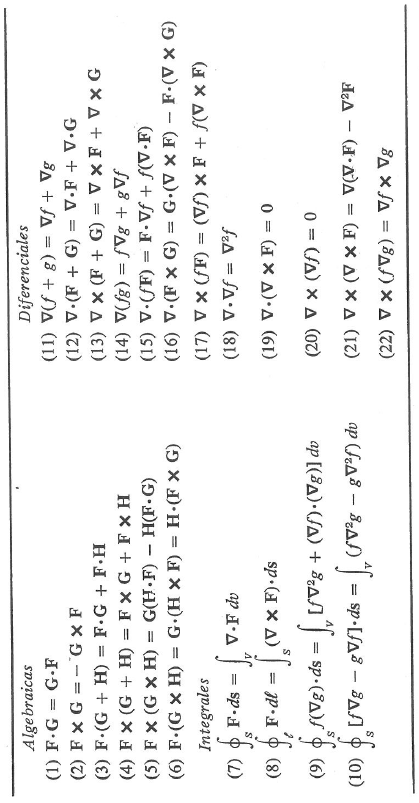
\includegraphics[scale=0.7, angle=-90]{Waves/waves_f4.png}
\end{figure}

\subsection{Teoremas integrales de Green}

Recordemos el teorema de la divergencia

\begin{equation*}
\oiint_s \mathbf{F} \cdot d \mathbf{S} = \iiint_v (\nabla \cdot \mathbf{F}) \ d V
\end{equation*}

si se especializa este teorema a una clase determinada de funciones vectoriales y obtener las identidades conocidas como los teoremas de Green.

Sea $\mathbf{F}$ un campo vectorial tal que $\mathbf{F}= f \mathbf{\nabla}g$, es decir, $\mathbf{F}$ es campo conservativo.

Aplicamos el teorema de divergencia a este campo

\begin{equation*}
\oiint_s (f \mathbf{\nabla}g) \cdot d \mathbf{S} = \iiint_v (\nabla \cdot (f \mathbf{\nabla}g)) \ d V
\end{equation*}

usamos las propiedades vectoriales y queda

\begin{equation*}
\oiint_s (f \mathbf{\nabla}g) \cdot d \mathbf{S} =  \iiint_v \left( f \nabla^2 g + (\nabla f) \cdot (\nabla g) \right) \ d V
\end{equation*}

Es la primera identidad integral de Green.

Por su parte, sea $\mathbf{G}= g \nabla f$, aplicando teorema de divergencia, obtenemos

\begin{equation*}
\oiint_s (g \mathbf{\nabla}f) \cdot d \mathbf{S} =  \iiint_v \left( g \nabla^2 f + (\nabla g) \cdot (\nabla f) \right) \ d V
\end{equation*}

Restamos las anteriores

\begin{eqnarray*}
\oiint_s (f \mathbf{\nabla}g) \cdot d \mathbf{S} - \oiint_s (g \mathbf{\nabla}f) \cdot d \mathbf{S} &=& \iiint_v \left( f \nabla^2 g + (\nabla f) \cdot (\nabla g) \right) \ d V - \iiint_v \left( g \nabla^2 f + (\nabla g) \cdot (\nabla f) \right) \ d V \\
\oiint_s (f \mathbf{\nabla}g - g \mathbf{\nabla}f ) \cdot d \mathbf{S} &=& \iiint_v \left( f \nabla^2 g + (\nabla f) \cdot (\nabla g) - \left( g \nabla^2 f + (\nabla g) \cdot (\nabla f) \right) \right) dV \\
\oiint_s (f \mathbf{\nabla}g - g \mathbf{\nabla}f ) \cdot d \mathbf{S} &=& \iiint_v \left( f \nabla^2 g - g \nabla^2 f \right) dV \\
\end{eqnarray*}

Esta es el teorema simétrico de Green.

Este teorema sirve para probar y demostrar que si dos funciones tienen el mismo rotacional y divergencia, entonces estas dos funciones son iguales y por lo tanto es una funcipon única.

\subsection{Ecuaciones de onda para campos eléctricos y magnéticos}

Volvamos a escribir las ecuaciones de Maxwell:

\begin{eqnarray*}
\nabla \cdot (\epsilon_0 \mathbf{E}) &=& \rho_v \\
\nabla \cdot \mathbf{B} &=& 0 \\
\nabla \times \mathbf{E} &=& - \frac{\partial \mathbf{B}}{\partial t} \\
\nabla \times \frac{\mathbf{B}}{\mu_0} &=& \mathbf{J} + \epsilon_0 \frac{\partial \mathbf{E}}{\partial t} 
\end{eqnarray*}

Tomemos rotacional a ambos lados de 

\begin{eqnarray*}
\nabla \times \mathbf{E} &=& - \frac{\partial \mathbf{B}}{\partial t} \\
\nabla \times \left( \nabla \times \mathbf{E} \right) &=& \nabla \times \left( - \frac{\partial \mathbf{B}}{\partial t} \right) \\
\nabla \times \left( \nabla \times \mathbf{E} \right) &=& - \frac{\partial \left( \nabla \times \mathbf{B} \right)}{\partial t} \\
\nabla \times \left( \nabla \times \mathbf{E} \right) &=& - \frac{\partial}{\partial t} \left( \nabla \times \mathbf{B} \right)
\end{eqnarray*}

De la otra ecuación de Maxwell:

\begin{eqnarray*}
\nabla \times \frac{\mathbf{B}}{\mu_0} &=& \mathbf{J} + \epsilon_0 \frac{\partial \mathbf{E}}{\partial t} \\
\nabla \times \mathbf{B} &=& \mu_0 \mathbf{J} +  \mu_0 \epsilon_0 \frac{\partial \mathbf{E}}{\partial t} 
\end{eqnarray*}

y reemplazamos $\nabla \times \mathbf{B}$:

\begin{eqnarray*}
\nabla \times \left( \nabla \times \mathbf{E} \right) &=& - \frac{\partial}{\partial t} \left( \mu_0 \mathbf{J} +  \mu_0 \epsilon_0 \frac{\partial \mathbf{E}}{\partial t}  \right) \\
\nabla \times \left( \nabla \times \mathbf{E} \right) + \mu_0 \epsilon_0 \frac{\partial^2 \mathbf{E}}{\partial t^2} &=& -\mu_0 \frac{\partial \mathbf{J}}{\partial t}
\end{eqnarray*}

Vemos que esta es una ecuación diferencial parcial vectorial que se conoce como ecuación no homogénea vectorial de onda para el espacio vacío. 

Realizando un procedimiento y susticuciones similares para las otras ecuaciones de Maxwell llegamos a una segunda ecuación de 

\begin{equation*}
\nabla \times \left( \nabla \times \mathbf{B} \right) + \mu_0 \epsilon_0 \frac{\partial^2 \mathbf{B}}{\partial t^2} = \mu_0 \nabla \times \mathbf{J}
\end{equation*}

Si el campo eléctrico no es divergente ($\nabla \cdot \mathbf{E}=0$), entonces el término $\nabla \times (\nabla \times \mathbf{E})$ se reduce a $-\nabla^2 \mathbf{E}$; más aún, si el campo no es divergente en la región, significa que la región está libre de cargas ($\rho_v=0$). Adicionalmente sabemos que el campo magnético es siempre divergente, entonces podemos escribir las ecuaciones de onda de la siguiente forma

\begin{eqnarray*}
\nabla^2 \mathbf{E} - \mu_0 \epsilon_0 \frac{\partial^2 \mathbf{E}}{\partial t^2} &=& \mu_0 \frac{\partial \mathbf{J}}{\partial t} \\
\nabla^2 \mathbf{B} - \mu_0 \epsilon_0 \frac{\partial^2 \mathbf{B}}{\partial t^2} &=& -\mu_0 \nabla \times \mathbf{F}
\end{eqnarray*}


Si la región es el espacio vacío, es decir, $\mathbf{J}=0$, se pueden obtener las siguientes ecuaciones 

\begin{eqnarray*}
\nabla^2 \mathbf{E} - \mu_0 \epsilon_0 \frac{\partial^2 \mathbf{E}}{\partial t^2} &=& 0 \\
\nabla^2 \mathbf{B} - \mu_0 \epsilon_0 \frac{\partial^2 \mathbf{B}}{\partial t^2} &=& 0
\end{eqnarray*}

las cuales son las ecuaciones homogéneas vectoriales de onda para el espacio vacío.\\


Miremos el caso para coordenadas cartesianas:

\begin{eqnarray*}
\nabla^2 E_x - \mu_0 \epsilon_0 \frac{\partial^2 E_x}{\partial t^2} &=& 0 \\
\nabla^2 E_y - \mu_0 \epsilon_0 \frac{\partial^2 E_y}{\partial t^2} &=& 0 \\
\nabla^2 E_z - \mu_0 \epsilon_0 \frac{\partial^2 E_z}{\partial t^2} &=& 0 
\end{eqnarray*}

\begin{eqnarray*}
\nabla^2 B_x - \mu_0 \epsilon_0 \frac{\partial^2 B_x}{\partial t^2} &=& 0 \\
\nabla^2 B_y - \mu_0 \epsilon_0 \frac{\partial^2 B_y}{\partial t^2} &=& 0 \\
\nabla^2 B_z - \mu_0 \epsilon_0 \frac{\partial^2 B_z}{\partial t^2} &=& 0 
\end{eqnarray*}

Si tenemos los campos $\mathbf{E}=e^{i \omega t}\mathbf{\hat{E}}$, entonces obtenemos

\begin{eqnarray*}
\nabla^2 \hat{E}_x + \omega^2 \mu_0 \epsilon_0 \hat{E}_x &=& 0 \\
\nabla^2 \hat{E}_y + \omega^2 \mu_0 \epsilon_0 \hat{E}_y &=& 0 \\
\nabla^2 \hat{E}_z + \omega^2 \mu_0 \epsilon_0 \hat{E}_z &=& 0
\end{eqnarray*}

\begin{eqnarray*}
\nabla^2 \hat{B}_x + \omega^2 \mu_0 \epsilon_0 \hat{B}_x &=& 0 \\
\nabla^2 \hat{B}_y + \omega^2 \mu_0 \epsilon_0 \hat{B}_y &=& 0 \\
\nabla^2 \hat{B}_z + \omega^2 \mu_0 \epsilon_0 \hat{B}_z &=& 0
\end{eqnarray*}

Las soluciones más simples de esas ecuaciones escalares de onda son ondas planas uniformes que comprenden hasta solo dos componentes.

\subsection{Ondas planas uniformes en es espacio vacío} \label{Ondas_planas_uniformes_en_es_espacio_vacio}

Las propiedades de simplificación son que las soluciones se prestan al sistema de coordenadas rectangulares y que el número de componentes de canpo se reduce a un mínimo de dos. con estas propiedades, las soluciones de onda mas simples son ondas planas uniformes.

las ondas tienen la propiedad de que en cualquier instante fijo los campos eléctricos y magnéticos son uniformes sobre superficies planas. Los planos son escogidos arbitrariamente. de manera que están definidos para $z=C$ constante lo que equivale a expresar que las variaciones espaciales de los campos eléctrico y magnético son cero sobre los planos $z=C$ esto conlleva a lo siguiente:

\begin{enumerate}
    \item Los campos no dependen de $x$ ni de $y$, es es que $\frac{\partial }{\partial x} = \frac{\partial }{\partial y} = 0$ para todas las componentes del campo.
    \item En toda la región las densidades de carga y de corriente son cero.
\end{enumerate}

Con estas suposiciones, las ecuaciones de maxwell quedan de la siguiente forma

\begin{eqnarray*}
\nabla \cdot (\epsilon_0 \mathbf{\hat{E}} ) = 0 \\
\nabla \cdot \mathbf{\hat{B}} = 0 \\
\nabla \times \hat{E} = - i \omega \mathbf{\hat{B}} \\
\nabla \times \frac{\mathbf{\hat{B}}}{\mu_0} = i \omega \epsilon_0 \mathbf{\hat{E}}
\end{eqnarray*}

Sabemos que combinando las ecuaciones anteriores llegamos a 

\begin{eqnarray*}
\nabla^2 \mathbf{\hat{E}} + \omega^2 \mu_0\epsilon_0 \mathbf{\hat{E}} = 0\\
\nabla^2 \mathbf{\hat{B}} + \omega^2 \mu_0\epsilon_0 \mathbf{\hat{B}} = 0
\end{eqnarray*}


Teniendo en cuenta las suposiciones anteriores de que  $\frac{\partial }{\partial x} = \frac{\partial }{\partial y} = 0$ , podemos ver para las rotacionales lo siguiente

\begin{equation*}
\nabla \times \mathbf{\hat{E}} = - i \omega (\mathbf{a}_x \hat{B}_x + \mathbf{a}_y \hat{B}_y  + \mathbf{a}_z \hat{B}_z )
\end{equation*}

conlleva a 

\begin{eqnarray*}
-\frac{\partial \hat{E}_y}{\partial z} = - i \omega \hat{B}_x \\
\frac{\partial \hat{E}_x}{\partial z} = - i \omega \hat{B}_y \\
\hat{B}_z = 0
\end{eqnarray*}

y de forma similar 


\begin{eqnarray*}
-\frac{\partial \hat{B}_y}{\partial z} = i \omega \mu_0\epsilon_0 \hat{E}_x \\
\frac{\partial \hat{B}_x}{\partial z} = i \omega \mu_0\epsilon_0 \hat{E}_y \\
\hat{E}_z = 0
\end{eqnarray*}

Como se puede ver, no existe componente en $z$ de ningún campo, y que se obtienen dos pares independientes de campos soluciones. 

Por ejemplo, si hacemos $\hat{E}_y = 0$, obtenemos que se eliminan dos de las cuatro ecuaciones, y se obtiene el siguiente sistema

\begin{eqnarray*}
\frac{\partial \hat{E}_x}{\partial z} = - i \omega \hat{B}_y \\
-\frac{\partial \hat{B}_y}{\partial z} = i \omega \mu_0\epsilon_0 \hat{E}_x 
\end{eqnarray*}


Combinando estas ecuaciones para obtener una ecuación que solo dependa de uno de los componentes, obtenemos la siguiente ecuación diferencial


\begin{equation*}
\frac{\partial^2 \hat{E}_x}{\partial z^2} + \omega^2 \mu_0\epsilon_0 \hat{E}_x = 0
\end{equation*}

Esta ecuación es de una sola variable y su solución está dada por

\begin{eqnarray*}
\hat{E_x}(z) = \hat{C_1} e^{-i \beta_0 z} + \hat{C_2} e^{i \beta_0 z}
\end{eqnarray*}

donde el término $\beta_0$ se denomina \textit{constante de fase}

\begin{equation*}
\beta_0 = \omega \sqrt{\mu_0 \ \epsilon_0 }
\end{equation*}

estas soluciones exponenciales complejas son representaciones de ondas de amplitud constante que viajan en las direcciones positiva y negativa de z. Los coeficientes complejos $ \hat{C_1}$ y $ \hat{C_2}$ deben tener las unidades de voltios por metro para denotar amplitudes complejas de las ondas que viajan en sentido positivo y negativo del eje $z$. por tanto empleamos una notación más adecuada

\begin{equation*}
\hat{E_x} (z) = \hat{E}_m^+ e^{-i \beta_0 z} + \hat{E}_m^- e^{i \beta_0 z}
\end{equation*}

Ahora reemplazando esta solución para determinar el campo magnético

\begin{eqnarray*}
\hat{B}_y &=& -\frac{1}{i \omega} \frac{\partial \hat{E}_x}{\partial z} \\
\hat{B}_y &=& -\frac{1}{i \omega} (- i \beta_0 \hat{E}_m^+ e^{-i \beta_0 z} + i \beta_0 \hat{E}_m^- e^{i \beta_0 z}) \\
\hat{B}_y &=& \frac{\beta_0}{\omega} \hat{E}_m^+ e^{-i \beta_0 z} - \frac{\beta_0}{\omega} \hat{E}_m^- e^{i \beta_0 z} \\
\hat{B}_y &=& \sqrt{\mu_0\epsilon_0} \hat{E}_m^+ e^{-i \beta_0 z} - \sqrt{\mu_0\epsilon_0} \hat{E}_m^- e^{i \beta_0 z}
\end{eqnarray*}

La parte real de la solución del campo eléctrico se puede expresar como

\begin{eqnarray*}
E_x(z,t) &=& \text{Re} \{ \hat{E}_x(x) e^{i \omega t} \}  \\
E_x(z,t) &=& E_m^+ \cos (\omega t - \beta_0 z + \phi^+) + E_m^- \cos (\omega t + \beta_0 z + \phi^-)
\end{eqnarray*}

Esto teniendo en cuenta que las constantes $\hat{E}_m^+$ y $\hat{E}_m^-$ sean números complejos cuyas fases (ángulos) son $\phi^+$ y $\phi^-$ respectivamente.

\begin{eqnarray*}
\hat{E}_m^+ = E_m^+ e ^(i \phi^+) \\
\hat{E}_m^- = E_m^- e ^(i \phi^-) 
\end{eqnarray*}


De manera similar tenemos la solución para el campo magnético 


\begin{eqnarray*}
B_x(z,t) &=& \sqrt{\mu_0\epsilon_0} E_m^+ \cos (\omega t - \beta_0 z + \phi^+) + \sqrt{\mu_0\epsilon_0} E_m^- \cos (\omega t + \beta_0 z + \phi^-)
\end{eqnarray*}

el factor de fase determina la longitud de onda, que significa la distancia que debe recorrer la onda para alzancar $2 \pi$ radianes.

\begin{equation*}
\beta_0 \lambda = 2 \pi
\end{equation*}


Por tanto, la longitud de onda es


\begin{equation*}
\lambda = \frac{2 \pi}{\beta_0} = \frac{2 \pi}{\omega \sqrt{\mu_0\epsilon_0}} = \frac{c}{m}
\end{equation*}


la velocidad de fase está dada por 


\begin{eqnarray*}
v_p &=& \frac{\omega}{\beta_0} \\
v_p &=& \frac{1}{\sqrt{\mu_0\epsilon_0}}
\end{eqnarray*}

Esta velocidad es la velocidad de la luz en el espacio vacío, $c$.


Si se define el campo de intensidad magnética $\mathbf{H} = \frac{\mathbf{B}}{\mu_0}$, se tiene que 

\begin{eqnarray*}
\frac{\hat{E}_x^+ (z)}{\hat{H}_y^+ (z)} = \mu_0 \ c = \sqrt{\frac{\mu_0}{\epsilon_0}} \equiv \eta_0 \approx 120 \pi \Omega \\
 = - \frac{\hat{E}_x^- (z)}{\hat{H}_y^- (z)}
\end{eqnarray*}

$\eta_0$ se define como la impedancia intrínseca de onda para el espacio vacío 


\section{Campos electromagnéticos para regiones materiales en estado de reposo}

\subsection{Conductividad eléctrica de los materiales}

El comportamiento de los campos se caracteriza por considerar tres efectos

\begin{enumerate}
    \item Conducción de carga eléctrica.
    \item Polarización eléctrica.
    \item Polarización magnética.
\end{enumerate}

esos efectos se describen de forma adecuada mediante tres parámetros: la conductividad eléctrica $\sigma$, la permitividad eléctrica $\epsilon$ y la permeabilidad magnética $\mu$.

los materiales pueden ser clasificados en función de sus propiedades de conducción eléctrica con aislantes, que esencialmente no posee ningún electrón libre para dar corriente bajo un campo eléctrico, y conductores; los cuales sí poseen una gran cantidad de electrones libres de órbitas externas para producir una corriente de conducción bajo un campo eléctrico. 

A escalas moleculares y atómicas, un sólido eléctricamente conductor se visualiza como una red de iones positivos en los que los electrones de la órbitas externas pueden moverse aleatoriamente. Sobre esta estructura están superpuestas agitaciones térmicas asociadas con la temperatura del conductor. Estos electrones libres se mueven con velocidades distribuidas aleatoriamente, con una velocidad media de

\begin{equation*}
v_d = \frac{1}{N} \sum_{i=1}^{N} v_i
\end{equation*}


promediada en cualquier instante sobre un número grande de partículas en el elemento de volumen. Esta velocidad promedio se denomina velocidad de deriva y es cero en ausencia de un campo eléctrico.

El tiempo llamado tiempo libre medio $\tau_c$, es el intervalo promedio entre las colisiones en un elemento de volumen. Cuando los electrones chocan con la red de iones, ceden en promedio un impulso $m v_d$ en el tiempo libre medio, y la razón promediada de transferencia de impulso a la red de iones por electrón es $\frac{m v_d}{\tau_c}$ N de fuerza, si se iguala esta con la fuerza debida a la ley de Lorentz, se tiene

\begin{equation*}
\frac{m \mathbf{v}_d}{\tau_c} = -e \mathbf{E}
\end{equation*}

 lo cual deja

 \begin{equation*}
\mathbf{v}_d = - \frac{e \tau_c}{m} \mathbf{E}
 \end{equation*}

 esta ecuación relaciona directamente la velocidad de deriva con el campo aplicado. Vemos que es proporcional al campo y que 

 \begin{equation*}
\mu_e = \frac{e \tau_e}{m} \frac{\text{m}^2}{\text{V-s}}
 \end{equation*}

 Rcordemos que la densidad de corriente está dada por 

 \begin{equation*}
\mathbf{J} = \rho_v \mathbf{v}_d
 \end{equation*}

 teniendo que $\rho_v = n e$, donde $n$ es la densidad de electrones libres por metro cúbico (número de $e^-$ por unidad de volumen), la anterior ecuación se escribe como sigue

 \begin{equation*}
\mathbf{J} = \rho_v \mathbf{v}_d = - n e \mathbf{v}_d = \frac{n e^2}{m} \tau_c
 \end{equation*}

 Vemos que la densidad de corriente es función lineal del campo eléctrico. 

 \begin{equation*}
\mathbf{J} = \sigma \mathbf{E}
 \end{equation*}

es la forma puntual de la ley de Ohm.


Teniendo en cuenta ña velocidad adicional de cambio del impulso promedio de la nube electrónicaen deriva en el conductor, la ecuación de la fuerza producida por el campo eléctrico se convierte en

\begin{equation*}
m \frac{d \mathbf{v}_d}{d t} + \frac{m}{\tau_c} \mathbf{v}_d = -e \mathbf{E}
\end{equation*}

lo cual da como resultado una solución para la velocidad de deriva 

\begin{equation*}
v_d = v_{d0} e^{-t/\tau_c}
\end{equation*}

el cual indica una respuesta transitoria de decaimiento o relajación en la velocidad de deriva al interrupir repentinamente el campo aplicado. Esta ecuación puede simplificarse si se supone $\mathbf{E}$ sinusoidal y su solución armónica en el tiempo implica que la conductividad se convierta en un número complejo. Sin embargo, para la mayoría de los casos esta conductividad siempre se asumirá real.


\subsection{Polarización eléctrica}

cuando un material dieléctrico está bajo un campo eléctrico, hay desplazamientos microscópicos de las uniones de cargas negativas y positivas. Este fenómeno se denomina polarización dieléctrica y puede darse de distintas formas:

\begin{itemize}
    \item Polarización electrónica, en que la nube de electrones negativos de un átomo se desplaza de la posición de equilibrio con respecto a su núcleo atómico.
    \item Polarizaciín iónica, en que los iones positivos y negativos de una molécula se desplazan en presencia del campo.
    \item Polarización de orientación, que ocurre en materiales con dipolos eléctricos permanentes, se orientan en la dirección del campo aplicado.
\end{itemize}

Si se imprime un campo eléctrico en el material, en el núcleo positivo y la nuve electrónica negativa se ejercerán fuerzas de lorentz $\mathbf{F}_e = q \mathbf{E}$, para producir desplazamientos de ambos sistemas de partículas. El equilibrio de desplazamiento se logra cuando las fuerzas atractivas internas de Coulomb de los dipolos internos balancean las fuerzas aplicadas.

El momento $\mathbf{p}_i$ del el i-ésimo par desplazado en una colección de dipolos polarizados está definido por

\begin{equation*}
\mathbf{p}_i = q \ \mathbf{d}_i \text{C \ m}
\end{equation*}

aquí $q$ denota la carga positiva del dipolo y $\mathbf{d}$ es la seperación vectorial del mismo, dirigida de la carga negativa a la positiva.

El momento dipolar eléctrico promedio por unidad de volumen se denomina campo de polarización eléctrica y se denota por $\mathbf{P}$ se define mediante

\begin{equation*}
\mathbf{P} = \frac{\sum_{i=1}^{N}\mathbf{p}_i}{\Delta v} = \frac{\sum_{i=1}^{N} q_i \mathbf{d}_i}{\Delta v} \text{ C/} \text{m}^2
\end{equation*}

El elemento de volumen tiene $N$ dipolos eléctricos.

si el material tiene una densidad de gargas positiva y negativa de $\rho_+$ y $\rho_-$ entonces el campo de polarización se escribe


\begin{equation*}
\mathbf{P} = \frac{\sum_{i=1}^{N}\mathbf{p}_i}{\Delta v} = \frac{\sum_{i=1}^{N} q_i \mathbf{d}_i}{\Delta v} = \frac{N q}{\Delta v} \frac{\sum_{i=1}^{N} \mathbf{d}_i}{N} \text{ C/} \text{m}^2 = \rho_+ \ \mathbf{d}
\end{equation*}


donde $\mathbf{d}$ es el vector promedio de las orientaciones de los dipolos.

El exceso de carga de polarización presente en un materia l tiene la consecuencia de modificar la ecuación de Maxwell de manera que 

\begin{equation*}
\nabla \cdot (\epsilon_0 \mathbf{ \mathbf{E} + \mathbf{P}}) = \rho_v
\end{equation*}

Sea el campo $\mathbf{D}\equiv \epsilon_0 \mathbf{E} + \mathbf{P}$, entonces


\begin{equation*}
\nabla \cdot D = \rho_v
\end{equation*}

Los experimentos revelan que muchas sustancias dieléctricas son especialmente lineales, lo que significa que 

\begin{equation*}
\mathbf{P} = \chi_e \epsilon_0 \mathbf{E}
\end{equation*}

donde se define a $\chi_e$ como la susceptibilidad eléctrica del material, quedando la ecuiación de maxwell

\begin{equation*}
\nabla \cdot ((1 + \chi_e)\epsilon_0 \mathbf{E}) = \rho_v
\end{equation*}


 o 

 \begin{equation*}
\mathbf{D} = (1 + \chi_e)\epsilon_0 \mathbf{E}
 \end{equation*}

y se define $\epsilon_r \equiv 1 + \chi_e$ como la \textit{permitividad relativa o constante dieléctrica} del material. Si se define finalmente la permitividad del material como

\begin{equation*}
\epsilon \equiv \epsilon_0 \ \epsilon_r
\end{equation*}

se tiene el campo 

\begin{equation*}
\mathbf{D} = \epsilon \mathbf{E}
\end{equation*}

quedando finalmente la ecuación de Maxwell para campos eléctricos en materiales

\begin{eqnarray*}
\nabla \cdot \mathbf{(\epsilon \mathbf{E})} = \rho_v \\
\nabla \cdot \mathbf{D} = \rho_v \text{ C/m}^3
\end{eqnarray*}


En general los materiales no son lineales del todo, aunque lo son en un rango amplio de $\mathbf{E}$. Sin embargo, si el campo eléctrico es lo suficientemente intenso, se puede producir dislocaciones moleculares en el material, llamadas rupturas dieléctricas. En un material no lineal, la susceptibilidad eléctrica es función de la magnitud de $\mathbf{E} = E$, quedando 

\begin{equation*}
\mathbf{P} = \chi (E) \epsilon_0 \mathbf{E}
\end{equation*}


\subsubsection{Densidad de corriente en la polarización}

si el campo es variable, también lo será la polarización. Entonces los desplazamientos de los constituyentes de cargas positivas en una dirección junto con las cargas negativas que se mueven en la dirección opuesta, dan lugar a desplazamientos de cargas a través de secciones transversales del material, identificables como corrientes a través de esas mismas secciones. El cambio en el tiempo del campo de polarización se define como $\mathbf{J}_p$

\begin{equation*}
\mathbf{J}_p \equiv \frac{\partial \mathbf{P}}{\partial t} \text{A/m}^2
\end{equation*}

Es la densidad de corriente de polarización eléctrica.

La forma integral de estas leyes para las regiones materiales son 

\begin{eqnarray*}
\oiint_S \mathbf{D} \cdot d \mathbf{s} = \iiint_v \rho_v \ dv \text{ C} \\
\oiint_S \mathbf{P} \cdot d \mathbf{s} = \iiint_v \rho_p \ dv \text{ C} 
\end{eqnarray*}

\subsubsection{Condiciones de frontera espacial para campos normales}

Es necesario estudiar el comportamiento de los campos en las regiones de cambio de material. En estos problemas es necesario definir todas las condiciones de frontera en la interacciones de los materiales. Estas condiciones de frontera se determinan a partir de las integrales de Maxwell. 

Se puede usar 

\begin{equation*}
\oiint_S \mathbf{D} \cdot d \mathbf{s} = \iiint_v \rho_v \ dv \text{ C} 
\end{equation*}

a través de una superficie cerrada construida apropiadamente para comparar las componentes normales de $\mathbf{D}$ que aparecen justo a ambos lados de la interacción de los materiales con distintas permitividades ($\epsilon_1$ $\epsilon_2$), se define una superficie cerrada en forma de caja redonda de altura $\delta h$ y áreas en las tapas $\Delta s$ de manera que se penetran ambas regiones a cada lado de la interacción :

\begin{figure}[H]
    \centering
    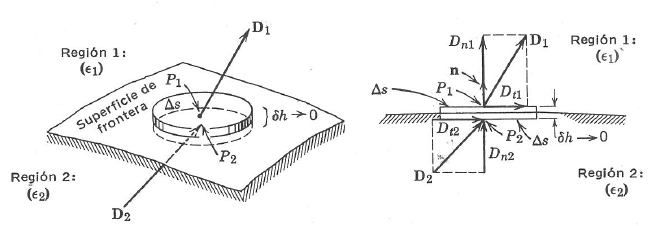
\includegraphics[scale=0.5]{Waves/waves_f5.png}
\end{figure}

Llamando $\mathbf{D}_1$ y $\mathbf{D}_2$ a los campos en puntos dentro de las regiones 










\textbf{SE DEJA PENDIENTE CONTINUAR CON LAS CONDICIONES DE FRONTERA PARA LOS CAMPOS EN MATERIALES JONHK PAG 141}



























































 
\section{Teoría electromagnética para ondas}



El fenómeno electromagnético a nivel macroscópico está descrito por las ecuaciones de Maxwell, publicadas en el año 1873. Su trabajo resumió el estado de la teoría electromagnética y realizó una hipótesis a partir de consideraciones teóricas la existencia de corrientes de desplazamiento eléctrica, lo cual llevó al descubrimiento experimental de Hertz de la propagación electromagnétic. El trabajo de maxwell se basó en una gran cantidad de conocimiento previo empírico y teórico que desarrollaron Gauss, Ampere, Faraday , entre otros. Recordemos, nuevamente, las ecuaciones de Maxwell para los campos eléctrico y magnético.


Volvamos nuevamente a las formas generales de las ecuaciones de Maxwell en su forma diferencial

\begin{eqnarray*}
\nabla \times \mathbf{\mathcal{\bar{E}}} &=& - \frac{\partial \mathcal{\bar{B}}}{\partial t} - \mathcal{\bar{M}} \\
\nabla \times \mathbf{\mathcal{\bar{H}}} &=& \frac{\partial \mathcal{\bar{D}}}{\partial t} + \mathcal{\bar{J}} \\
\nabla \cdot \mathcal{\bar{D}} &=& \rho \\
\nabla \cdot \mathcal{\bar{B}} &=& 0
\end{eqnarray*}

Los campos se describen como sigue

\begin{itemize}
    \item $\mathcal{\bar{E}}$ es el campo eléctrico en voltios por metro (V/m)
    \item $\mathcal{\bar{H}}$ es el campo magnético en amperios por metro (A/m)
    \item $\mathcal{\bar{D}}$ es la densidad de flujo eléctrico, en coulombs por metro cuadrado (C/m2)
    \item $\mathcal{\bar{B}}$ es la densidad de flujo magnético, en webers por metro cuadrado (Wb/m2)
    \item $\mathcal{\bar{N}}$ es una medida ficticia de densidad de corriente magnética, en voltios por metro cuadrado (V/m2)
    \item $\mathcal{\bar{J}}$ Es la densidad de corriente eléctrica, en amperios por metro cuadrado (A/m2)
    \item $\rho$ es la densidad volumétrica de carga eléctrica, en Coulombs por metro cúbico (C/m3)
\end{itemize}

Las fuentes de los campos electromagnéticos son las densidades de corrientes, y de carga (últimas tres de la lista arriba). En el espacio vacío se tiene

\begin{eqnarray*}
\mathcal{\bar{B}} &=& \mu_0 \mathcal{\bar{H}} \\
\mathcal{\bar{D}} &=& \epsilon_0 \mathcal{\bar{E}} 
\end{eqnarray*}

\begin{itemize}
    \item $\mu_0 = 4 \pi \times 10 ^{-7}$ es la permeabilidad magnética del espacio libre, en henrios por metro (H/m)
    \item $\epsilon_0 = 8.854 \times 10^{-125}$ es la permitividad eléctrica del espacio libre, en faradios por metro (F/m) 
\end{itemize}

Volvamos ahiora a las formas integrales de las ecuaciones de Maxwell

\begin{eqnarray*}
\oint_S \mathcal{\bar{D}} \cdot d \bar{s} &=& \int_V \rho \ dv = Q \\
\oint_S \mathcal{\bar{B}} \cdot d \bar{s} &=& 0 \\
\oint_C \mathcal{\bar{E}} \cdot d \bar{l} &=& - \frac{\partial}{\partial t} \int_S \mathcal{\bar{B}} \cdot d \bar{s} - \int_S \mathcal{\bar{M}} \cdot \bar{s} \\
\oint_C \mathcal{\bar{H}} \cdot d \bar{l} &=& \frac{\partial}{\partial t} \int_S \mathcal{\bar{D}} \cdot d \bar{s} + \int_S \mathcal{\bar{J}} \cdot \bar{s} 
\end{eqnarray*}

El campo eléctrico se puede expresar como dependiente del tiempo, armónica y en estado estable; por tal, un campo eléctrico sinusoidal que viaja en la dirección $x$ es 

\begin{eqnarray*}
\mathcal{\bar{E}}(x,y,z,t) = \mathcal{E}_x \hat{x} \cos(\omega t + \phi)  
\end{eqnarray*}

Donde $\mathcal{E}_x$ denota la amplitud del campo. El fasor correspondiente al campo estará dado por

\begin{equation*}
\bar{E}(x,y,z) = \hat{x} \ \mathcal{E}_x \ e^{i \phi} 
\end{equation*}

Se asume una representación de fasores cosenoidal, de modo que 


\begin{equation*}
\mathcal{\bar{E}} (x,y,z,t) = \text{Re} \{ \bar{E}(x,y,z) e^{i \omega t} \}
\end{equation*}


Es importante, al tratar con potencia y energía, tener el cuenta el promedio cuadrático. Teniendo el campo

\begin{equation*}
\mathcal{\bar{E}} = \mathcal{E}_x \cos (\omega t + \phi_x) \hat{x} + \mathcal{E}_y \cos (\omega t + \phi_y) \hat{y} + \mathcal{E}_z \cos (\omega t + \phi_z) \hat{z}
\end{equation*}

El cual tiene la forma fasorial 

\begin{equation*}
\mathcal{\bar{E}} = \mathcal{E}_x e^{i \phi_x} \hat{x} + \mathcal{E}_y e^{i \phi_y} \hat{y} + \mathcal{E}_z e^{i \phi_z} \hat{z}
\end{equation*}

Tiene un valor medio cuadrático de 

\begin{eqnarray*}
|\mathcal{\bar{E}}|_{\text{avg}}^2 &=& \frac{1}{T} \int_0^T \mathcal{\bar{E}} \cdot \mathcal{\bar{E}} \ dt \\
&=& \frac{1}{T} \int_0^T \left(  \mathcal{E}_x^2 \cos^2 (\omega t + \phi_x) + \mathcal{E}_y^2 \cos^2 (\omega t + \phi_y) + \mathcal{E}_z^2 \cos^2 (\omega t + \phi_z) \right) \ dt \\ 
&=& \frac{1}{2} (\mathcal{E}_x^2 + \mathcal{E}_y^2) + \mathcal{E}_z^2)  \\
&=& \frac{1}{2} |\bar{E}|^2 \\
&=& \frac{1}{2} \bar{E} \ \bar{E}^*
\end{eqnarray*}

El valor RMS del campo es

\begin{equation*}
|\bar{E}|_{RMS} = \frac{|\bar{E}|}{\sqrt{2}}
\end{equation*}

Bajo la dependencia del tiempo, las ecuaciones en forma diferencial son

\begin{eqnarray*}
\nabla \times \bar{E} &=& - i \omega \bar{B} - \bar{M} \\
\nabla \times \bar{H} &=& \ i \omega \bar{D} + \bar{J} \\
\nabla \cdot \bar{D} &=& \rho \\
\nabla \cdot \bar{B} &=& 0
\end{eqnarray*}


\subsection{Campos en materiales y las condiciones de frontera}

En un material dieléctrico, cuando se aplica un campo eléctrico, causa la polarización de los átomos o moléculas del material, se crean momentos dipolares que aumentan el flujo de desplazamiento total $\bar{D}$. La polarización adicional se llama $\bar{P}$ y queda el campo como

\begin{equation*}
\bar{D} = \epsilon_0 \bar{E} + \bar{P}
\end{equation*}

Si el medio (material) es lineal, la polarización está relacionada linealmente con el campo aplicado, la constante de proporción se llama susceptibilidad eléctrica, se tiene

\begin{equation*}
\bar{P} = \epsilon_0 \chi_e \bar{E}
\end{equation*}

la susceptibilidad puede ser un número complejo, la ecuación de campo queda como sigue

\begin{eqnarray*}
\bar{D} &=& \epsilon_0 \bar{E} + \epsilon_0 \chi_e \bar{E} \\
\bar{D} &=& \epsilon_0 \bar{E} (1+ \chi_e) \\
\bar{D} &=& \epsilon \bar{E}
\end{eqnarray*}

\begin{equation*}
\epsilon_0(1+ \chi_e) = \epsilon = \epsilon' - i \epsilon''
\end{equation*}

La parte imaginaria de la permitividad del medio es debida a las pérdidas en el medio en forma de calor por el amortiguamiento de los momentos dipolares vibrantes. Esta parte imaginaria debe ser negativa por conservación de la energía. Las pérdidas en el material dieléctrico pueden ser consideradas como equivalentes a las pérdidas en los conductores. En un material con conductividad $\sigma$, existirá en él una densidad de corriente de conducción dada por 

\begin{equation*}
\bar{J} = \sigma \bar{E}
\end{equation*}

La ecuación rotacional de Maxwell

\begin{eqnarray*}
\nabla \times \bar{H} &=& i \omega \bar{D} + \bar{J} \\
&=& i \omega \epsilon \bar{E} +\sigma \bar{E} \\
&=& i \omega \epsilon' \bar{E} + (\omega \epsilon'' + \sigma) \bar{E} \\
&=& i \omega \left( \epsilon' - i \epsilon'' - i \frac{\sigma}{\omega} \bar{E} \right)
\end{eqnarray*}

Donde se ha visto que las pérdidas debidas al amortiguamiento dieléctrico ($\omega \epsilon''$) son indistinguibles de las debidas a la conductividad ($\sigma$). El termino $\omega \epsilon'' + \sigma$ se considera como la conductividad total efectiva.\\

Otra cantidad de interés es la denominada \textit{tangente de pérdida} definida como 

\begin{equation*}
\tan \delta = \frac{\omega \epsilon'' + \sigma}{\omega \epsilon'0}
\end{equation*}

la cual se ve como la relación entre la parte real y la parte imaginaria de la corriente de desplazamiento total. Los materiales de microondas son caracterizados usualmente especificando la permitividad real relativa (constante dieléctrica) $\epsilon_r$, con $\epsilon' = \epsilon_0 \epsilon_r$, y la tangente de pérdida en función de la frecuencia. 

Hasta este momento se ha asumido que el vector de momentos dipolares $\bar{P}$ está en la misma dirección que el campo eléctrico. Para los meteriales con este comportamiento se les conoce como isotrópicos. No todos los materiales son isotrópicos, son denominados anisotrópicos y se caracterizan por tener una relaxión más complicada entre $\bar{D}$ y $\bar{P}$. La relación lineal más general entre estos vectores toma la forma de un tensor de rango 2, el cual se escribe de forma matricial de la siguiente forma:

\begin{equation*}
\left[
\begin{aligned}
    D_x \\
    D_y \\
    D_z
\end{aligned}
\right] = 
\left[
\begin{aligned}
    \epsilon_{xx} && \epsilon_{xy}  && \epsilon_{xz}  \\
    \epsilon_{yx} && \epsilon_{yy}  && \epsilon_{yy}  \\
    \epsilon_{zx} && \epsilon_{zy}  && \epsilon_{zz}  
\end{aligned}
\right]
\left[
\begin{aligned}
    E_x \\
    E_y \\
    E_z
\end{aligned}
\right] = [\epsilon]
\left[
\begin{aligned}
    E_x \\
    E_y \\
    E_z
\end{aligned}
\right]
\end{equation*}

Como ejemplos de materiales anisotrópicos podemos mencionar algunas estructuras cristalinas y gases ionizados. \\

Las mismas relaciones pueden hacerse para los campos magnéticos 

\begin{equation*}
\bar{B} = \mu_0 (1 + \chi_m) \bar{H} = \mu \bar{H}
\end{equation*}

\begin{equation*}
\left[
\begin{aligned}
    B_x \\
    B_y \\
    B_z
\end{aligned}
\right] = 
\left[
\begin{aligned}
    \mu_{xx} && \mu_{xy}  && \mu_{xz}  \\
    \mu_{yx} && \mu_{yy}  && \mu_{yy}  \\
    \mu_{zx} && \mu_{zy}  && \mu_{zz}  
\end{aligned}
\right]
\left[
\begin{aligned}
    H_x \\
    H_y \\
    H_z
\end{aligned}
\right] = [\mu]
\left[
\begin{aligned}
    H_x \\
    H_y \\
    H_z
\end{aligned}
\right]
\end{equation*}

\subsubsection*{Campos en una interfaz material general}


\begin{figure}[H]
    \centering
    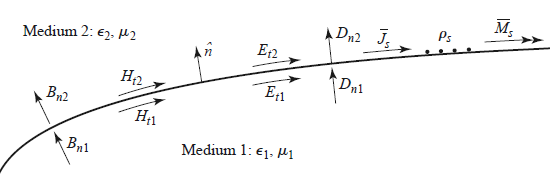
\includegraphics[scale=0.6]{Waves/waves_f6.png}
\end{figure}

Para determinar las condiciones de frontera se hace uso de las formas integrales de las ecuaciones de Maxwell. De esta manera se encuentran las condiciones que deben cumplirse para los campos normales y tangenciales a la interfaz. 

Aplicamos la integral de Maxwell de Gauss en un volumen como se indica en la imagen siguiente

\begin{figure}[H]
    \centering
    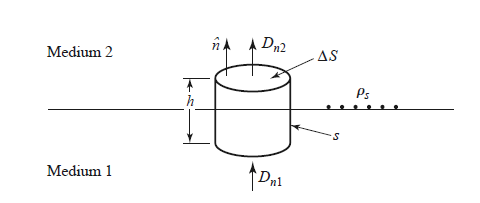
\includegraphics[scale=0.6]{Waves/waves_f7.png}
\end{figure}

\begin{equation*}
\oint_S \bar{D} \cdot d \bar{s} = \int_V \rho \ d v
\end{equation*}

Cuando se hace el límite de $h \to 0$, la contribución tangencial del campo $\bar{D}$ se hace cero, por tanto solamente habrá componente normal sobre el área circular $\Delta S$ por tanto

\begin{equation*}
\left( D_{n2} - D_{n1} \right) \Delta S =  \Delta S \rho_s
\end{equation*}

En el límite, la densidad volumétrica de carga se convierte en densidad superficial. 

\begin{equation*}
D_{n2} - D_{n1} =  \rho_s
\end{equation*}

De manera vectorial se puede escribir

\begin{equation*}
\hat{n} \cdot \left( \bar{D}_{2} - \bar{D}_{1} \right) = \rho_s
\end{equation*}

haciendo una argumentación similar para el campo $B$, se tiene

\begin{equation*}
\hat{n} \cdot \bar{B}_2 = \hat{n} \cdot \bar{B}_1
\end{equation*}

Para la parte tangencial del campo eléctrico, vemos la fórmula integral 

\begin{equation*}
\oint_C \bar{E} \cdot d \Bar{l} = - i \omega \int_S \bar{B} \cdot d \bar{s} - \int_S \bar{M} \cdot d \bar{s}
\end{equation*}

aplicada a la línea cerrada:

\begin{figure}[H]
    \centering
    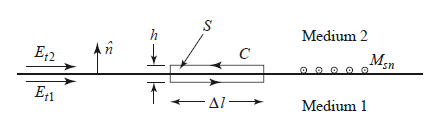
\includegraphics[scale=0.6]{Waves/waves_f8.png}
\end{figure}

nuevamente hacemos e límite $h \to 0$, el área de la superficie $\Delta l \ h$ tiende a cero, por lo que la integral de superficie de $\Bar{B}$ desaparece. Sin embargo, la contribución del campo $\bar{M}$ puede no anularse si en la superficie existe una densidad de corriente superficial magnética: de modo que se puede escribir mediante la función delta de dirac:

\begin{equation*}
\bar{M} = \bar{M}_s \delta (h)
\end{equation*}

por tanto, la ecuación queda

\begin{eqnarray*}
\Delta l E_{t1} - \Delta l E_{t2} &=& - \Delta l M_s \\
 E_{t1} - E_{t2} &=& - M_s
\end{eqnarray*}

o, vectorialmente

\begin{equation*}
\left( \bar{E}_2 - \bar{E}_1 \right) \times \hat{n} = \bar{M}_s
\end{equation*}

De manera similaar para los campos magnéticos

\begin{equation*}
\hat{n} \times \left( \bar{H}_2 - \bar{H}_1 \right) = \bar{J}_s
\end{equation*}

Estas son las expresiones más generales para las condiciones de frontera

\subsubsection*{Campos en la interfaz dieléctrica}

Cuando los materiales son dieléctricos, no existen cargas libres ni corrientes superficiales, por tanto las condiciones de frontera quedarán

\begin{eqnarray*}
\hat{n} \cdot \bar{D_1} &=& \hat{n} \cdot \bar{D_2} \\
\hat{n} \cdot \bar{B_1} &=& \hat{n} \cdot \bar{B_2} \\
\hat{n} \times \bar{E_1} &=& \hat{n} \times \bar{E_1} \\
\hat{n} \times \bar{H_1} &=& \hat{n} \times \bar{H_2} \\
\end{eqnarray*}

\subsubsection*{Campos en la interfaz con un conductor perfecto}

Cuando se tiene un material conductor con una alta conductividad (se puede asumir $\sigma \to \infty$) todos los campos son nulos dentro del material condcutor perfecto. En este tipo de casos se tendrá que las condiciones de frontera son:


\begin{eqnarray*}
\hat{n} \cdot \bar{D} &=& \rho_s \\
\hat{n} \cdot \bar{B} &=& 0 \\
\hat{n} \times \bar{E} &=& 0 \\
\hat{n} \times \bar{H} &=& \bar{J_s}
\end{eqnarray*}

\subsection{Ecuación de onda y soluciones básicas para ondas planas}

en un medio homogéneo, isotrópico, lineal y sin fuentes de campos, la ecuación de maxwel puede llegarse a simlpificar en 

\begin{eqnarray*}
\nabla^2 \bar{E} + \omega^2 \ \mu \epsilon  \bar{E} \\
\nabla^2 \bar{H} + \omega^2 \ \mu \epsilon  \bar{H}
\end{eqnarray*}

Se define la constante de propagación $\beta=\omega \sqrt{\mu \epsilon}$, y se asume la solución, como se mostró en la sección \ref{Ondas_planas_uniformes_en_es_espacio_vacio}, se tiene la solución (para ondas viajantes en la direción x)

\begin{equation*}
E_x(z) = E^+ e^{i \beta z} + E^- e^{-i \beta z}
\end{equation*}

o escrito de otra forma

\begin{equation*}
\mathcal{E} (x,t) = E^+ \cos (\omega t - \beta z) + E^- \cos (\omega t + \beta z)
\end{equation*}

Nuevamente tenemos la velocidad de propagación

\begin{equation*}
v_p = \frac{\omega}{\beta} = \frac{1}{\sqrt{\mu \ \epsilon}}
\end{equation*}

Y también la longitud de onda para las ondas planas

\begin{equation*}
\lambda = \frac{2 \pi}{\beta} = \frac{2 \pi v_p}{\omega } = \frac{v_p}{f}
\end{equation*}

Veamos el campo magnético, que por ecuación de maxwell es

\begin{equation*}
H_y = \frac{i}{\omega \mu} \frac{\partial E_x}{\partial z} = \frac{1}{\eta} (  E^+ e^{-i \beta z} - E^- e^{i \beta z} )
\end{equation*}

donde $\eta = \sqrt{\mu / \epsilon}$ se denomina la impedancia intrínseca del medio.

\subsubsection*{Medio con pérdidas}

Cuando el medio tiene pérdidas, tenemos que hay una conductividad $\sigma$ la ecuación de onda queda

\begin{equation*}
\nabla^2 \bar{E} + \omega^2 \ \mu \epsilon \left( 1 - i \frac{\sigma}{\omega \epsilon} \right) \bar{E} = 0
\end{equation*}

En este caso se tiene que la constante de propagación cambia de ser $\beta^2=\omega^2 \mu \epsilon$ a $\omega^2 \mu \epsilon (1-i(\sigma/\omega \epsilon))$ y se tiene un número complejo de onda o constante compleja de propagación de onda

\begin{equation*}
\gamma = \alpha + i \beta = i \omega \sqrt{\mu \epsilon} \sqrt{1-i \frac{\sigma}{\omega \epsilon}}
\end{equation*}

en este caso se asume una solución para una onda plana en dirección $x$ par que quede la solución

\begin{equation*}
E_x(z) = E^+ e^{-\gamma z} + E^- e^{\gamma z}
\end{equation*}

La onda que viaja en el sentido positivo de $x$ tiene el factor

\begin{eqnarray*}
e^{- \gamma z} = e^{- \alpha z} e ^{-i \beta z}
\end{eqnarray*}
Note que de esta manera el campo se atenúa en el espacio $\alpha$.

El campo magnético en este caso será

\begin{equation*}
H_y = \frac{i}{\omega \mu} \frac{\partial E_x}{\partial z} = \frac{1}{\eta} (  E^+ e^{-i \gamma z} - E^- e^{i \gamma z} )
\end{equation*}

Aquí la impedancia intrínseca del medio está dada por

\begin{equation*}
\eta = \frac{i \omega \mu}{\gamma}
\end{equation*}

\subsubsection*{Medio es un conductor}

Si el medio es un conductor, podemos decir que su conductividad es muy alta, por tanto $\sigma \gg \omega \epsilon$, se puede hacer la aproximación de $\gamma$


\begin{equation*}
\gamma = \alpha + i \beta \approx i \omega \sqrt{\mu \epsilon} \sqrt{ \frac{\sigma}{i \omega \epsilon}} = (1 + i) \sqrt{\frac{\omega \mu \sigma}{2}}
\end{equation*}

\subsection{Solución general de las ondas planas}

veamos la ecuación de Helmholtz para el campo eléctrico en coordenadas rectangulares

\begin{equation*}
\nabla^2 \bar{E} + \beta_0^2 \Bar{E} = \frac{\partial^2 \Bar{E}}{\partial x^2} + \frac{\partial^2 \Bar{E}}{\partial y^2} + \frac{\partial^2 \Bar{E}}{\partial z^2} + \beta_0^2 \Bar{E} = 0
\end{equation*}

Esto da como resultado que para cada coordenada cartesiana

\begin{equation*}
 \frac{\partial^2 E_i}{\partial x^2} + \frac{\partial^2 E_i}{\partial y^2} + \frac{\partial^2 E_i}{\partial z^2} + \beta_0^2 E_i = 0
\end{equation*}

Esta ecuación diferencial parcial puede resolverse mediante el método de separación de variables. Se empieza por asumir que la solución para la componente del campo $E_x$ se puede escribir como el producto de

\begin{equation*}
E_x(x,y,z) = f(x)g(y)h(z)
\end{equation*}

la solución final de la ecuación diferencial estará dada por 

\begin{equation*}
\bar{E} = \bar{E}_0 e^{- i \ \bar{\beta} \cdot \bar{r}}
\end{equation*}

donde tenemos que 

\begin{equation*}
\bar{r} = \hat{x} x + \hat{y} y + \hat{z} z
\end{equation*}

Propiedades importantes de esta solución indican que el vector de las amplitudes del campo deben ser perpendiculares a la dirección en la que se propaga. 

\begin{equation*}
\bar{\beta} \cdot \bar{E}_0 = 0
\end{equation*}


El campo magnético está dado por

\begin{equation*}
\bar{H} = \frac{1}{\eta_0} \hat{n} \times \bar{E}
\end{equation*}

\subsubsection*{Polarización circular de las ondas}

sabemos que las ondas viajan hacia la dirección perpendicular de la amplitud de $\Bar{E}$ y $\bar{H}$. Hasta ahora hemos visto que la orientación del vector $\bar{E}$ no cambia con el tiempo, es decir, siempre es perpendicular a $\hat{x}$, propagándose en la dirección $\hat{z}$. Este tipo de onda plana se considera una \textit{onda de polarización lineal}. Para este caso se tendrá que $\bar{H}$ será perpendicular a $\hat{y}$. \\

Existe una polarización de las ondas planas en las que la dirección del campo $\bar{E}$ también cambia con el tiempo. Esto quiere decir que el vector rota sobre planos $xy$ con una velocidad angular. Como se puede observar en la siguiente imagen

\begin{figure}[H]
    \centering
    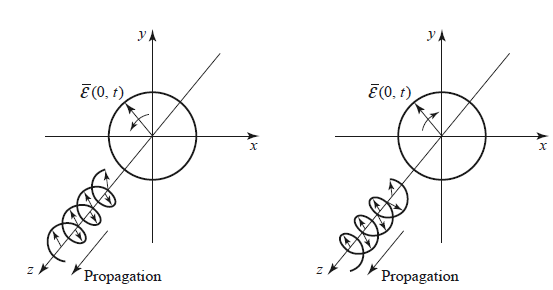
\includegraphics[scale=0.6]{Waves/wave_f9.png}
\end{figure}

\subsection{Potencia y energía}

En general, una fuente de energía electromagnética establece campos que almacenan energía eléctrica y magnética, y transportan potencia que puede transmitirse o disiparse como pérdida. En el caso del estado estacionario sinusoidal, la energía eléctrica almacenada promedio en un volumen V se da por
 \begin{eqnarray*}
W_e &=& \frac{1}{4} \text{Re} \left\{ \int_V \bar{E} \cdot \bar{D}^* \ d v \right\} \\
W_m &=& \frac{1}{4} \text{Re} \left\{ \int_V \bar{H} \cdot \bar{B}^* \ d v \right\} 
 \end{eqnarray*}

Tanto para campos eléctricos como para campos magnéticos. Si el medio es isotrópico, lineal, homogéneo y sin pérdida, entonces la permitividad y permeabildiad son escalares reales y constantes, entonces las energías promedio almacenadas son

\begin{eqnarray*}
W_e &=& \frac{\epsilon}{4} \text{Re} \left\{ \int_V \bar{E} \cdot \bar{E}^* \ d v \right\} \\
W_m &=& \frac{\mu}{4} \text{Re} \left\{ \int_V \bar{H} \cdot \bar{H}^* \ d v \right\} 
 \end{eqnarray*}

 De aqui se puede derivar el teorema de Poynting, el cual lleva a la conservación de energía de campos electromagnéticos y fuentes.

 Partiendo de las ecuacioes diferenciales de maxwell y con algunas propiedades vectoriales, se concluye que

 \begin{equation*}
- \frac{1}{2} \int_V ( \bar{E} \cdot \bar{J}_s + \bar{H} \cdot \bar{M}_s  ) dv = \frac{1}{2} \oint_S \left( \bar{E} \times \bar{H}^* \right) \cdot d \bar{s} + \frac{\sigma}{2} \int_V |\bar{E}|^2 d v + \frac{\omega}{2} \int_V (\epsilon'' |\bar{E}|^2 + \mu'' |\bar{H}|^2) d v + i \frac{\omega}{2}   \int_V (\mu' |\bar{H}|^2 - \epsilon' |\bar{E}|^2) d v
 \end{equation*}


Esta ecuación de balances de potencia es el teorema de Poynting. La integral de la parte izquierda de la ecuación representa la potencia compleja $P_s$ entregada por las fuentes de campo $\bar{J}_s$ y $\bar{M}_s$ dentro del volumen

\begin{equation*}
P_s = - \frac{1}{2} \int_V ( \bar{E} \cdot \bar{J}_s + \bar{H} \cdot \bar{M}_s  ) dv
\end{equation*}

Laprimera integral de la parte derecha de la ecuación representa el flujo de potencia compleja que sale de la superficie cerrada $S$, se define entoncdes el \textit{vector de Poynting} como $\bar{S}$

\begin{equation*}
\bar{S} =  \bar{E} \times \bar{H}^* 
\end{equation*}

por tanto este flujo de potencia se representa

\begin{equation*}
P_o = \frac{1}{2} \oint_S \left( \bar{E} \times \bar{H}^* \right) \cdot d \bar{s} = \frac{1}{2} \oint_S \bar{S} \cdot d \bar{s}
\end{equation*}

Las partes reales de las potencias $P_s$ y $P_o$ representan potencias promedio.

La segunda y tercera integral de la parte derecha de la ecuación son escalares reales que representan la potencia promedio disipada en el volumen $V$ debido a la conductividad y pérdidas dieléctricas y magnéticas. $P_l$

\begin{equation*}
P_l =  \frac{\sigma}{2} \int_V |\bar{E}|^2 d v + \frac{\omega}{2} \int_V (\epsilon'' |\bar{E}|^2 + \mu'' |\bar{H}|^2) d v 
\end{equation*}

Esta se denomina en algunas ocasiones como la ley de Joule. La última integral finalmente está relacionada con las energías electromagnéticas almacenadas, son potencias reactivas.

El teorema de Poynting se escribe nuevamente como sigue

\begin{equation*}
P_s = P_o + P_l + 2 i omega (W_e - W_e)
\end{equation*}

La potencia total entregada por las fuentes de ondas es la suma de la potencia transmitida a través de la superficie más la potencia disipada por pérdidas térmicas y electromagnéticas, más $2 \omega$ veces la potencia reactiva neta que se almacena en el volumen.

\subsubsection*{Potencia absorbida por un buen conductor}


En la vida practica las líneas de transmisión involucran conductores imperfectos, dando lugar a pérdidas de atenuación de campo y de potencia, así como generación de ruido. Para calcular estas pérdidas es necesario que se calcule la potencia disipada por estos conductores. Considere la siguiente geometría

\begin{figure}[H]
    \centering
    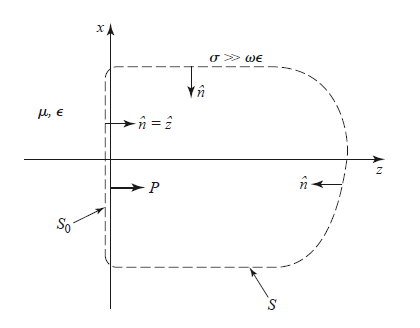
\includegraphics[]{Waves/waves_f10.png}
\end{figure}

Representando la interfaz de un medio sin pérdidas y un conductor bueno. Un campo es incidente en la dirección $z<0$ y penetra en el conductor en $z>0$. La potencia real promedio que entra a la sección de volumen $V$ del conductor definida por el área transversal $S_0$ en la interfaz y el área $S$ dentro del conductor es 

\begin{equation*}
P_{avg} = \frac{1}{2} \text{Re} \int_{S_0+S} \bar{E} \times \bar{H}^* \cdot \hat{n} d s
\end{equation*}

Dado que las ondas son planas, van en dirección $\hat{z}$; además, el rápido decaimiento de los campos dentro de un material conductor también da lugar a que la contriución de estos en la región $S$ sea despreciable. Esto deja como resultado que la potencia sea

\begin{equation*}
P_{avg} = \frac{1}{2} \text{Re} \int_{S_0} \bar{E} \times \bar{H}^* \cdot \hat{z} d s
\end{equation*}

simplificamos

\begin{eqnarray*}
\hat{z} \cdot (\bar{E} \times \bar{H}^*) &=& (\hat{z} \times \bar{E}) \cdot  \bar{H}^* \\
&=& \eta \bar{H} \cdot  \bar{H}^* 
\end{eqnarray*}

Si $R_s = \text{Re} \eta = \sqrt{\frac{\omega \mu}{2 \sigma}}$, la potencia queda

\begin{equation*}
P_{avg} = \frac{1}{2} \frac{R_s}{2} \int_{S0} |\bar{H}|^2 \ ds
\end{equation*}

$R_s$ se define como la resistencia de superficie del conductor

\subsection{Reflexión de ondas planas de una interfaz de medios}

Cuando una onda plana de campo eléctrico pasa del espacio libre a un medio con $\epsilon$, $\mu$ y $\sigma$, parte de la onda se transmitirá al materia, y otra parte se refleja en la dirección opuesta:

\begin{figure}[H]
    \centering
    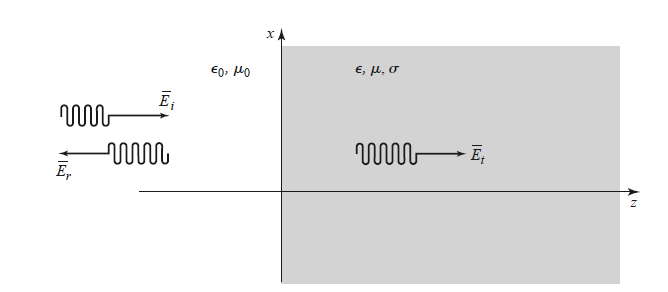
\includegraphics[scale=0.6]{Waves/waves_f11.png}
\end{figure}

Los campos incidentes son

\begin{eqnarray*}
\bar{E}_i &=& \hat{x} E_0 e^{- i \beta_0 z} \\
\bar{H}_i &=& \hat{y} \frac{1}{\eta_0} E_0 e^{- i \beta_0 z}
\end{eqnarray*}

Con amplitud $E_0$ arbitraria.

Las ondas reflejadas son 

\begin{eqnarray*}
\bar{E}_r &=& \hat{x} \Gamma E_0 e^{+ i \beta_0 z} \\
\bar{H}_r &=& - \hat{y} \frac{1}{\eta_0} \Gamma E_0 e^{+ i \beta_0 z}
\end{eqnarray*}

donde $\Gamma$ se denomina el \textbf{coeficiente de refexión} de la interfaz o medio. El signo positivo de la exponencial es un indicador de la dirección de propagación de la onda hacia $z$ negativo. \\

Los campos transmitidos al material están dados por

\begin{eqnarray*}
\bar{E}_t &=& \hat{x} \ T \ E_0 \ e^{- \gamma z} \\
\bar{H}_t &=& \hat{y} \ \frac{1}{\eta} T \ E_0 \ e^{-\gamma z}
\end{eqnarray*}

donde la constante de propagación es 

\begin{equation*}
\gamma = \alpha + i \beta = i \omega \sqrt{\mu \epsilon} \sqrt{1- i \sigma / \omega \epsilon}
\end{equation*}

y la impedancia del medio es

\begin{equation*}
\eta = \frac{i \omega \mu}{\gamma}
\end{equation*}

En este caso se tiene un problema de frontera, se tiene que los campos son continuos en la interfaz de los materiales, por tanto se tiene como condición de frontera

\begin{eqnarray*}
1 + \Gamma = T \\
\frac{1 - \Gamma}{\eta_0} = \frac{T}{\eta}
\end{eqnarray*}

La solución de el sistema es

\begin{eqnarray*}
\Gamma = \frac{\eta - \eta_0}{\eta + \eta_0} \\
T = \frac{2\eta}{\eta + \eta_0}
\end{eqnarray*}

Examinamos ahora las diferentes posibilidades para el material

\subsubsection*{Medio sin pérdidas}

Si el material es sin pérdidas, esto significa que $\sigma=0$ y que $\epsilon$ y $\mu$ son reales. Entonces la constante de propagación es imaginaria y está dada por 

\begin{equation*}
\gamma = i \beta = i \omega \sqrt{\epsilon \mu} = i \ \beta_0 \sqrt{\epsilon_r \mu_r}
\end{equation*}

La longitud de onda en el material es

\begin{equation*}
\lambda = \frac{2 \pi}{\beta} = \frac{2 \pi}{\omega \sqrt{\epsilon \mu}} = \frac{\lambda_0}{\sqrt{\epsilon_r \mu_r}}
\end{equation*}

la velocidad de fase (o de propagación= es 

\begin{equation*}
v_p = \frac{1}{ \sqrt{\epsilon \mu}} = \frac{c}{ \sqrt{\epsilon_r \mu_r}}
\end{equation*}

 Y la impedancia intrínseca del material será


\begin{equation*}
\eta = \sqrt{\frac{\mu}{\epsilon}} = \eta_0 \sqrt{\frac{\mu_r}{\epsilon_r}}
\end{equation*}

El vector de Poyting en la aregión $z<0$ es

\begin{eqnarray*}
\bar{S}^{-} = \bar{E} \times \bar{H}^* = (\bar{E}_i+\bar{E}_r) \times (\bar{H}_i+\bar{H}_r)^*
\end{eqnarray*}

Que conlleva a 

\begin{equation*}
\bar{S}^{-} = \hat{z} \ |E_0|^2 \frac{1}{\eta_0} \left(1-|\Gamma|^2 + 2 i \ \Gamma \sin (2 \beta_0 z)\right)
\end{equation*}

Dado $\Gamma \in \mathbb{R}$

ahora, para $z >0$, el vector de Poynting es

\begin{equation*}
\bar{S}^{+} = \bar{E}_t \times \bar{H_t}^* = \hat{z} \ \frac{|E_0|^2 \ |T|^2}{\eta}
\end{equation*}

esto puede reescribirse como

\begin{equation*}
\bar{S}^{+} = \hat{z} \ |E_0|^2 \ \frac{1}{\eta_0} \left(1-|\Gamma|^2 \right)
\end{equation*}

Ahora, note que los vectores deben ser iguales en la interfaz $\bar{S}^{+} = \bar{S}^{-}$ en $z=0$. La potencia real promedio en $z<0$ es

\begin{equation*}
P^{-} = \frac{1}{2} \text{Re} \left\{  \bar{S}^- \cdot \hat{z} \right\} = \frac{1}{2} \ |E_0|^2 \frac{1}{\eta_0} \left(1-|\Gamma|^2 \right) 
\end{equation*}

y en $z>0$ es

\begin{equation*}
P^{+} = \frac{1}{2} \text{Re} \left\{  \bar{S}^+ \cdot \hat{z} \right\} = \frac{1}{2} \ |E_0|^2 \frac{1}{\eta_0} \left(1-|\Gamma|^2 \right) = P^{-}
\end{equation*}

\subsubsection*{Medio conductor}

Aquí tenemos las siguientes propiedades

\begin{equation*}
\gamma = (1+i)\sqrt{\frac{\omega \ \mu \ \sigma}{2}} = (1+i) \frac{1}{\delta_s}
\end{equation*}

La impedancia intrínseca es 

\begin{equation*}
\eta =  (1+i)\sqrt{\frac{\omega \ \mu }{2\ \sigma}} = (1+i) \frac{1}{\sigma \ \delta_s}
\end{equation*}

El vector de poynting en $z=0$ es

\begin{equation*}
\bar{S}^{-}(z=0) = \hat{z} \ |E_0|^2 \frac{1}{\eta_0} \left( 1 - |\Gamma|^2 + \Gamma - \Gamma^{*} \right)
\end{equation*}

y para $z>0$

\begin{equation*}
\bar{S}^{+} = \hat{z} \ |E_0|^2 \frac{1}{\eta_0} \left( 1 - |\Gamma|^2 + \Gamma - \Gamma^{*} \right) e^{-2 \alpha z}
\end{equation*}

Las potencias reales promedio son

\begin{eqnarray*}
P^- &=& \frac{1}{2} \ |E_0|^2 \frac{1}{\eta_0} \left( 1 - |\Gamma|^2 +  \right) \\
P^+ &=& \frac{1}{2} \ |E_0|^2 \frac{1}{\eta_0} \left( 1 - |\Gamma|^2 +  \right) e^{-2 \alpha z}
\end{eqnarray*}

La densidad de corriente resultante en la reegión conductora está dada por 

\begin{equation*}
\bar{J}_t = \sigma \bar{E}_t = \hat{x} \sigma \ E_0 T e{- \gamma z} \text{A/m}^2
\end{equation*}

Y la potencia promedio real disipada o transmitida dentro de un volumen de sección transversal de $1\text{m}^2$ es

\begin{equation*}
P^t = \frac{\sigma \ |E_0|^2 \ |T|^2}{4 \ \alpha}
\end{equation*}

\subsubsection*{Conductor perfecto}

Ahora para un conductor perfecto se tiene que $\sigma \to \infty$, $\alpha \to \infty$, $\eta = 0$, $\delta_s \to 0$, $T \to 0$ y $\Gamma \to -1$  y se tiene que los campos decain infinitamente rápido en $z>0$, los campos fuera del conductor son

\begin{eqnarray*}
\bar{E} = \bar{E}_i + \bar{E}_r = - \hat{x} 2 \ i E_0 \sin (\beta_0 z) \\
\bar{H} = \bar{H}_i + \bar{H}_r = \hat{y} \frac{2}{\eta_0} E_0 \cos (\beta_0 z) \\
\end{eqnarray*}

El vector de Poynting es

\begin{equation*}
\bar{S}^- = -\hat{z} \ i \ \frac{4}{\eta_0} |E_0|^2 \sin (\beta_0 z) \cos (\beta_0 z)
\end{equation*}

La cual es puramente imaginaria y significa que no hay potencia entregada a un conductor perfecto. La corriente superficial se reduce a una densidad infinitesimalmente delgada 

\begin{equation*}
\bar{J}_s = \hat{x} \frac{2}{\eta_0} E_0
\end{equation*}


\section{Teoría de líneas de transmisión}


